\documentclass[a4paper,11pt]{article}
\usepackage[utf8]{inputenc}\usepackage[T1]{fontenc}
\usepackage[english]{babel}\usepackage{lmodern}\usepackage{microtype}
\usepackage{amsmath,amssymb}\usepackage{geometry}
\geometry{a4paper,left=2.2cm,right=2.2cm,top=2.0cm,bottom=2.0cm}
\usepackage{booktabs,array}\usepackage{xcolor}
\definecolor{bokug}{RGB}{0,135,60}\usepackage{tikz}
\usetikzlibrary{arrows.meta,calc}
\usepackage{fancyhdr}\pagestyle{fancy}
\renewcommand{\headrulewidth}{0.4pt}
\usepackage{enumitem}\setlength{\parindent}{0pt}\setlength{\parskip}{4pt}

\begin{document}
\fancyhead[L]{\small VU Mechanik – LAWI 100515 (PI)}\fancyhead[R]{\small SS 2026}\fancyfoot[C]{\thepage}
\begin{center}{\large\bfseries\color{bokug}University of Natural Resources and Life Sciences, Vienna (BOKU)}\\[2pt]{\large\bfseries VU Mechanik – LAWI 100515 (PI)}\\[4pt]Exam \textbf{Group A} \hfill Date: 26.06.2026\\[2pt]\rule{\linewidth}{0.4pt}\end{center}

\begin{center}\textbf{\large Model solution}\end{center}
\begin{center}
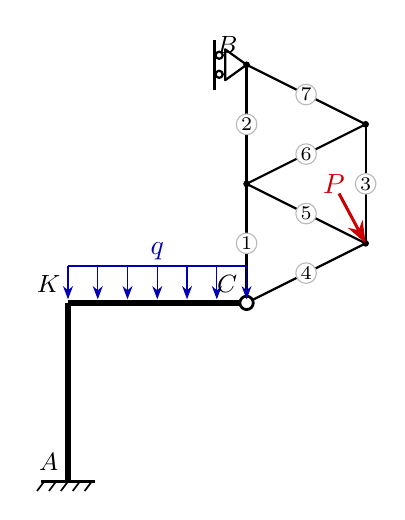
\begin{tikzpicture}[scale=0.756,>=Stealth,line join=round]
  \coordinate (P0) at (0.000,0.000);
  \coordinate (K) at (0.000,3.000);
  \coordinate (C) at (3.000,3.000);
  \coordinate (TO1) at (3.000,5.000);
  \coordinate (TO2) at (3.000,7.000);
  \coordinate (TU0) at (5.000,4.000);
  \coordinate (TU1) at (5.000,6.000);
  \draw[thick] (C) -- (TO1);
  \draw[thick] (TO1) -- (TO2);
  \draw[thick] (TU0) -- (TU1);
  \draw[thick] (C) -- (TU0);
  \draw[thick] (TU0) -- (TO1);
  \draw[thick] (TO1) -- (TU1);
  \draw[thick] (TU1) -- (TO2);
  \draw[line width=2.2pt] (P0) -- (K);
  \draw[line width=2.2pt] (K) -- (C);
  \fill (C) circle (1.6pt);
  \fill (TO1) circle (1.6pt);
  \fill (TO2) circle (1.6pt);
  \fill (TU0) circle (1.6pt);
  \fill (TU1) circle (1.6pt);
  \draw[fill=white,line width=1pt] (C) circle (3.2pt);
  \draw[line width=1.1pt] (-0.450,0.000) -- (0.450,0.000);
  \draw[line width=0.6pt] (-0.400,0.000) -- (-0.520,-0.160);
  \draw[line width=0.6pt] (-0.200,0.000) -- (-0.320,-0.160);
  \draw[line width=0.6pt] (0.000,0.000) -- (-0.120,-0.160);
  \draw[line width=0.6pt] (0.200,0.000) -- (0.080,-0.160);
  \draw[line width=0.6pt] (0.400,0.000) -- (0.280,-0.160);
  \draw[thick] (3.000,7.000) -- (2.640,7.260) -- (2.640,6.740) -- cycle;
  \draw[thick] (2.540,7.160) circle (0.06) (2.540,6.840) circle (0.06);
  \draw[line width=1pt] (2.460,7.420) -- (2.460,6.580);
  \node[circle,fill=white,draw=gray!55,inner sep=0.5pt,font=\scriptsize] at (3.000,4.000) {1};
  \node[circle,fill=white,draw=gray!55,inner sep=0.5pt,font=\scriptsize] at (3.000,6.000) {2};
  \node[circle,fill=white,draw=gray!55,inner sep=0.5pt,font=\scriptsize] at (5.000,5.000) {3};
  \node[circle,fill=white,draw=gray!55,inner sep=0.5pt,font=\scriptsize] at (4.000,3.500) {4};
  \node[circle,fill=white,draw=gray!55,inner sep=0.5pt,font=\scriptsize] at (4.000,4.500) {5};
  \node[circle,fill=white,draw=gray!55,inner sep=0.5pt,font=\scriptsize] at (4.000,5.500) {6};
  \node[circle,fill=white,draw=gray!55,inner sep=0.5pt,font=\scriptsize] at (4.000,6.500) {7};
  \draw[->,blue!70!black] (0.000,3.620) -- (0.000,3.060);
  \draw[->,blue!70!black] (0.500,3.620) -- (0.500,3.060);
  \draw[->,blue!70!black] (1.000,3.620) -- (1.000,3.060);
  \draw[->,blue!70!black] (1.500,3.620) -- (1.500,3.060);
  \draw[->,blue!70!black] (2.000,3.620) -- (2.000,3.060);
  \draw[->,blue!70!black] (2.500,3.620) -- (2.500,3.060);
  \draw[->,blue!70!black] (3.000,3.620) -- (3.000,3.060);
  \draw[blue!70!black,thick] (0.000,3.620) -- (3.000,3.620);
  \node[blue!70!black] at (1.500,3.870) {$q$};
  \draw[->,red!80!black,line width=1.1pt] (4.553,4.838) -- (5.000,4.000);
  \node[red!80!black] at (4.468,4.997) {$P$};
  \node[font=\small] at (0.000,0.000) [xshift=-7pt,yshift=7pt] {$A$};
  \node[font=\small] at (0.000,3.000) [xshift=-7pt,yshift=7pt] {$K$};
  \node[font=\small] at (3.000,3.000) [xshift=-7pt,yshift=7pt] {$C$};
  \node[font=\small] at (3.000,7.000) [xshift=-7pt,yshift=7pt] {$B$};
\end{tikzpicture}
\end{center}
\par\medskip\textbf{1.\ Static determinacy}\par Counting criterion $n=3k-(a+z)$ (bodies $k$, reactions $a$, interaction forces $z$):
\[ n=3k-(a+z)=3\cdot2-(4+2)=0\ \Rightarrow\ \text{statically determinate} \]
\par\medskip\textbf{2.\ Support reactions and hinge forces}\par
$A:\ R_x=1.5,\ R_y=24,\ M=54$\quad $B:\ R_x=-9.5,\ R_y=0$\par $C:\ H_x=-1.5,\ H_y=-15$
\par\medskip\textbf{3.\ Truss member forces}\par
\begin{center}\renewcommand{\arraystretch}{1.1}\begin{tabular}{c r l}
\toprule
Member & Force $S$ [kN] & Type \\
\midrule
  1 & -14.25 & compression \\
  2 & -4.75 & compression \\
  3 & 9.5 & tension \\
  4 & -1.68 & compression \\
  5 & 10.62 & tension \\
  6 & -10.62 & compression \\
  7 & 10.62 & tension \\
\bottomrule
\end{tabular}\end{center}
\begin{center}
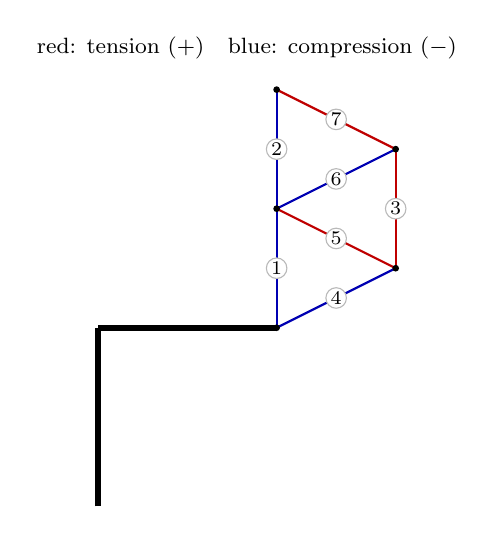
\begin{tikzpicture}[scale=0.756,>=Stealth,line join=round]
  \coordinate (P0) at (0.000,0.000);
  \coordinate (K) at (0.000,3.000);
  \coordinate (C) at (3.000,3.000);
  \coordinate (TO1) at (3.000,5.000);
  \coordinate (TO2) at (3.000,7.000);
  \coordinate (TU0) at (5.000,4.000);
  \coordinate (TU1) at (5.000,6.000);
  \draw[thick,blue!70!black] (C) -- (TO1);
  \draw[thick,blue!70!black] (TO1) -- (TO2);
  \draw[thick,red!75!black] (TU0) -- (TU1);
  \draw[thick,blue!70!black] (C) -- (TU0);
  \draw[thick,red!75!black] (TU0) -- (TO1);
  \draw[thick,blue!70!black] (TO1) -- (TU1);
  \draw[thick,red!75!black] (TU1) -- (TO2);
  \draw[line width=2pt] (P0) -- (K);
  \draw[line width=2pt] (K) -- (C);
  \fill (C) circle (1.6pt);
  \fill (TO1) circle (1.6pt);
  \fill (TO2) circle (1.6pt);
  \fill (TU0) circle (1.6pt);
  \fill (TU1) circle (1.6pt);
  \node[circle,fill=white,draw=gray!55,inner sep=0.5pt,font=\scriptsize] at (3.000,4.000) {1};
  \node[circle,fill=white,draw=gray!55,inner sep=0.5pt,font=\scriptsize] at (3.000,6.000) {2};
  \node[circle,fill=white,draw=gray!55,inner sep=0.5pt,font=\scriptsize] at (5.000,5.000) {3};
  \node[circle,fill=white,draw=gray!55,inner sep=0.5pt,font=\scriptsize] at (4.000,3.500) {4};
  \node[circle,fill=white,draw=gray!55,inner sep=0.5pt,font=\scriptsize] at (4.000,4.500) {5};
  \node[circle,fill=white,draw=gray!55,inner sep=0.5pt,font=\scriptsize] at (4.000,5.500) {6};
  \node[circle,fill=white,draw=gray!55,inner sep=0.5pt,font=\scriptsize] at (4.000,6.500) {7};
  \node[font=\footnotesize] at (2.50,7.70) {red: tension $(+)$\quad blue: compression $(-)$};
\end{tikzpicture}
\end{center}
\par\medskip\textbf{4.\ Section-force diagrams of the beams}\par
\begin{center}
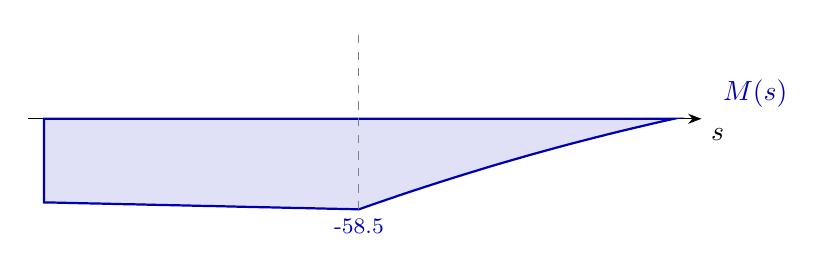
\begin{tikzpicture}[>=Stealth]
  \draw[->] (-0.2,0) -- (8.35,0) node[below right]{$s$};
  \filldraw[fill=blue!70!black!12,draw=blue!70!black,thick] (0,0) -- plot coordinates {(0.000,-1.062) (0.167,-1.065) (0.333,-1.069) (0.500,-1.073) (0.667,-1.076) (0.833,-1.080) (1.000,-1.084) (1.167,-1.087) (1.333,-1.091) (1.500,-1.095) (1.667,-1.098) (1.833,-1.102) (2.000,-1.106) (2.167,-1.109) (2.333,-1.113) (2.500,-1.117) (2.667,-1.121) (2.833,-1.124) (3.000,-1.128) (3.167,-1.132) (3.333,-1.135) (3.500,-1.139) (3.667,-1.143) (3.833,-1.146) (4.000,-1.150) (4.000,-1.150) (4.167,-1.091) (4.333,-1.034) (4.500,-0.977) (4.667,-0.921) (4.833,-0.867) (5.000,-0.813) (5.167,-0.760) (5.333,-0.708) (5.500,-0.657) (5.667,-0.606) (5.833,-0.557) (6.000,-0.509) (6.167,-0.461) (6.333,-0.415) (6.500,-0.369) (6.667,-0.324) (6.833,-0.281) (7.000,-0.238) (7.167,-0.196) (7.333,-0.155) (7.500,-0.115) (7.667,-0.076) (7.833,-0.037) (8.000,0.000)} -- (8.000,0) -- cycle;
  \draw[gray,dashed,thin] (4.000,-1.15) -- (4.000,1.15);
  \node[below,blue!70!black,font=\footnotesize] at (4.000,-1.150) {-58.5};
  \node[blue!70!black,right] at (8.50,0.32) {$M(s)$};
\end{tikzpicture}\\[5pt]
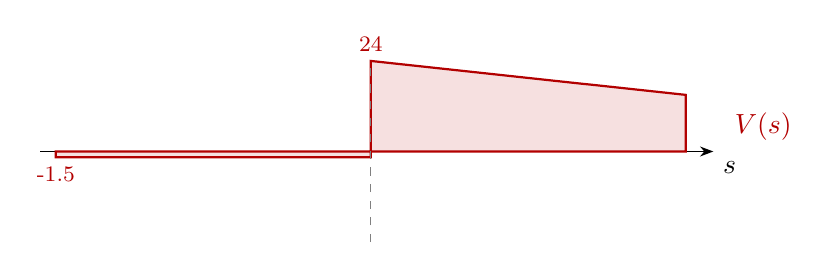
\begin{tikzpicture}[>=Stealth]
  \draw[->] (-0.2,0) -- (8.35,0) node[below right]{$s$};
  \filldraw[fill=red!70!black!12,draw=red!70!black,thick] (0,0) -- plot coordinates {(0.000,-0.072) (0.167,-0.072) (0.333,-0.072) (0.500,-0.072) (0.667,-0.072) (0.833,-0.072) (1.000,-0.072) (1.167,-0.072) (1.333,-0.072) (1.500,-0.072) (1.667,-0.072) (1.833,-0.072) (2.000,-0.072) (2.167,-0.072) (2.333,-0.072) (2.500,-0.072) (2.667,-0.072) (2.833,-0.072) (3.000,-0.072) (3.167,-0.072) (3.333,-0.072) (3.500,-0.072) (3.667,-0.072) (3.833,-0.072) (4.000,-0.072) (4.000,1.150) (4.167,1.132) (4.333,1.114) (4.500,1.096) (4.667,1.078) (4.833,1.060) (5.000,1.042) (5.167,1.024) (5.333,1.006) (5.500,0.988) (5.667,0.970) (5.833,0.952) (6.000,0.934) (6.167,0.916) (6.333,0.898) (6.500,0.880) (6.667,0.862) (6.833,0.845) (7.000,0.827) (7.167,0.809) (7.333,0.791) (7.500,0.773) (7.667,0.755) (7.833,0.737) (8.000,0.719)} -- (8.000,0) -- cycle;
  \draw[gray,dashed,thin] (4.000,-1.15) -- (4.000,1.15);
  \node[above,red!70!black,font=\footnotesize] at (4.000,1.150) {24};
  \node[below,red!70!black,font=\footnotesize] at (0.000,-0.072) {-1.5};
  \node[red!70!black,right] at (8.50,0.32) {$V(s)$};
\end{tikzpicture}\\[5pt]
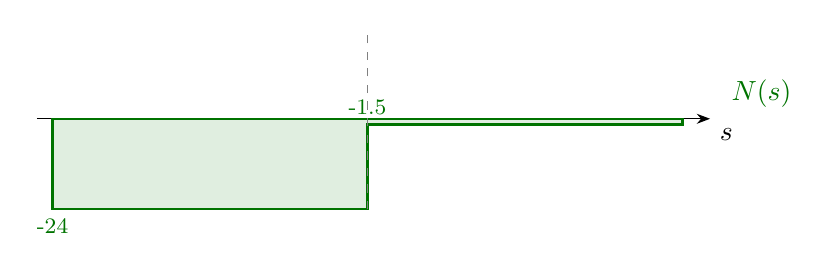
\begin{tikzpicture}[>=Stealth]
  \draw[->] (-0.2,0) -- (8.35,0) node[below right]{$s$};
  \filldraw[fill=green!45!black!12,draw=green!45!black,thick] (0,0) -- plot coordinates {(0.000,-1.150) (0.167,-1.150) (0.333,-1.150) (0.500,-1.150) (0.667,-1.150) (0.833,-1.150) (1.000,-1.150) (1.167,-1.150) (1.333,-1.150) (1.500,-1.150) (1.667,-1.150) (1.833,-1.150) (2.000,-1.150) (2.167,-1.150) (2.333,-1.150) (2.500,-1.150) (2.667,-1.150) (2.833,-1.150) (3.000,-1.150) (3.167,-1.150) (3.333,-1.150) (3.500,-1.150) (3.667,-1.150) (3.833,-1.150) (4.000,-1.150) (4.000,-0.072) (4.167,-0.072) (4.333,-0.072) (4.500,-0.072) (4.667,-0.072) (4.833,-0.072) (5.000,-0.072) (5.167,-0.072) (5.333,-0.072) (5.500,-0.072) (5.667,-0.072) (5.833,-0.072) (6.000,-0.072) (6.167,-0.072) (6.333,-0.072) (6.500,-0.072) (6.667,-0.072) (6.833,-0.072) (7.000,-0.072) (7.167,-0.072) (7.333,-0.072) (7.500,-0.072) (7.667,-0.072) (7.833,-0.072) (8.000,-0.072)} -- (8.000,0) -- cycle;
  \draw[gray,dashed,thin] (4.000,-1.15) -- (4.000,1.15);
  \node[above,green!45!black,font=\footnotesize] at (4.000,-0.072) {-1.5};
  \node[below,green!45!black,font=\footnotesize] at (0.000,-1.150) {-24};
  \node[green!45!black,right] at (8.50,0.32) {$N(s)$};
\end{tikzpicture}\\[10pt]
\end{center}
\end{document}